
%(BEGIN_QUESTION)
% Copyright 2010, Tony R. Kuphaldt, released under the Creative Commons Attribution License (v 1.0)
% This means you may do almost anything with this work of mine, so long as you give me proper credit

Beregn hva voltmeteret vil vise når det kobles til terminalene i RTD-hodet, hvis transmitteren i denne 3-leder RTD-kretsen bruker en strømkilde på 0.2 mA for å "eksitere" RTD-kretsen:

$$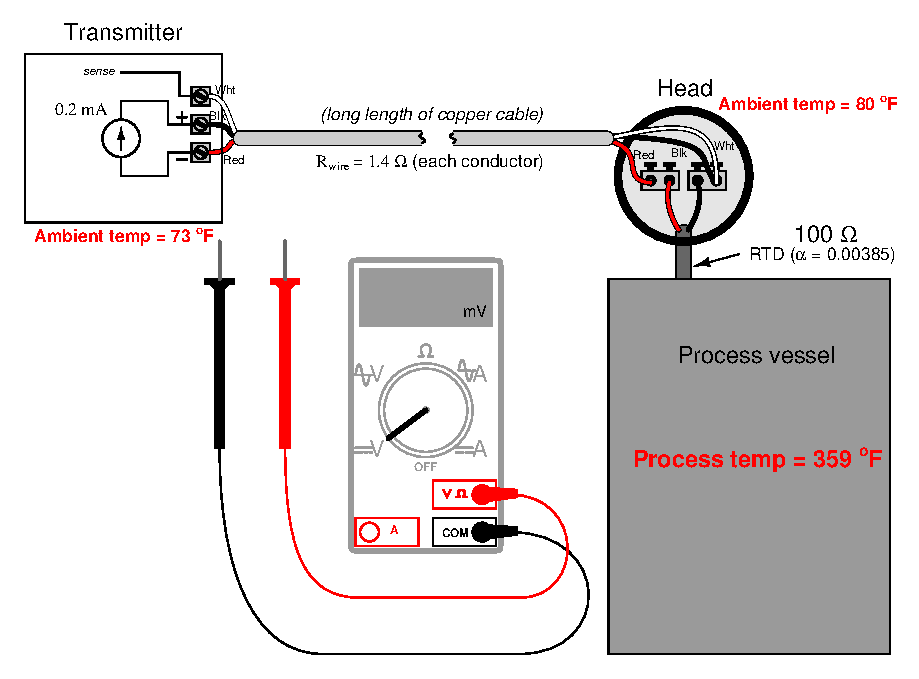
\includegraphics[width=15.5cm]{i00637x01.eps}$$

$V_{meter}$ = \underbar{\hskip 50pt} millivolt

\underbar{file i00637no}
%(END_QUESTION)





%(BEGIN_ANSWER)

$V_{meter}$ = {\bf 33.818} millivolt (basert på tabell)

\vskip 10pt

$V_{meter}$ = {\bf 33.988} millivolt (basert på formel)

%(END_ANSWER)





%(BEGIN_NOTES)

{\bf Denne oppgaven er ment for eksamen, ikke arbeidsark.}

%(END_NOTES)
